\section{Electrical and Wiring}

	The wiring diagram on the following page(Figure ~\ref{fig:WiringDiagram}) shows electrical layout of the system. The DoodleBot has two major groups of components - the electronics and control components sit in the DoodleBot Control Enclosure and the electromechanical components are mounted to the DoodleBot CNC Frame - that are interfaced by a 12-wire loom and a 2-wire loom broken by two connectors.
	
	\subsection{Connectors and Loom}
	
	\subsection{Voltage Dividers}
		The direction signals are produced from the PLC's embedded output on pins 0 and 1 at 24V. The AMCI SMD23 needs to read these signals as a +5V differential signal across its terminals.
		
		Because the AMCI SMD23 direction input is a digital signal (ie, high impedance input), we can use a simple voltage divider circuit to produce the correct voltage. The PLC embedded output can produce a maximum of 500mA per pin and requires a minimum of 1mA per pin while in the on-state to operate at 24V (going below this current limit causes the voltage to quickly drop to 0V).
		
		Choosing resistors of 820\Omega and 220\Omega in the voltage dividers gives a 5.08V output across the 220\Omega resistor. The voltage divider draws 2.3mA, which is within the operating specification of the embedded output.
	\subsection{Solenoid Driver}
		The pull type solenoid used in the Z-axis operation (drawing head) is designed to operate at 12V. It has a resistance of 58\Omega and an unknown inductance. In steady state operation it draws 207mA and consumes 6W. The solenoid can be modelled as an R-L circuit: an off-on transition will have current start at 0 and slowly ramp up to 207mA. In an on-off transition, there will be a spikes of negative current which gradually reduces to zero.
		
		The PLC embedded output can produce a maximum of 500mA per pin and requires a minimum of 1mA per pin while in the on-state to operate at 24V (going below this current limit causes the voltage to quickly drop to 0V).
		
		Due to the transient behaviour of the solenoid, a voltage divider cannot be used. Instead an STMicroelectronics L7812 Linear Voltage Regulator in TO220 packaging is used to perform a 24V-12V DC-DC conversion. 6W is lost as heat in the L7812, so a heatsink is used.
		
		Due to the minimum current requirement of the PLC output, a TIP31C bipolar junction transistor (BJT) is used as the solenoid switch (a field effect transistor (FET) would not work since it would not draw enough current to allow the PLC to operate normally).
		
		There is an additional requirement that the minimum current through the base of the BJT is enough to drive 207mA through the solenoid. The TIP31C datasheet shows that with a collector-emitter current of 1A, the minimum DC current gain is 25. So at least 8.28mA is required through the base. A more conservative value of 20mA is chosen by placing a 1.2k\Omega resistor in between the PLC output and BJT base.
		
		To allow the inductor to discharge quickly (and without damaging other components), a flyback diode is put across the Solenoid Driver Output in reverse orientation. In the on-off transition, the reverse current will have an alternate path to follow and energy will dissipate as heat in the solenoid and diode.
		
		
	\subsection{Kill Switch}
		The DoodleBot features a kill switch (emergency stop switch) mounted to Control Enclosure that disconnects the power supply's GND output from all the powered components. It should be noted that the power supply itself continues to operate and certain reactive components may retain their charge and as such, the kill switch should only be used in emergencies.


\begin{landscape}
		\vspace*{\fill}
		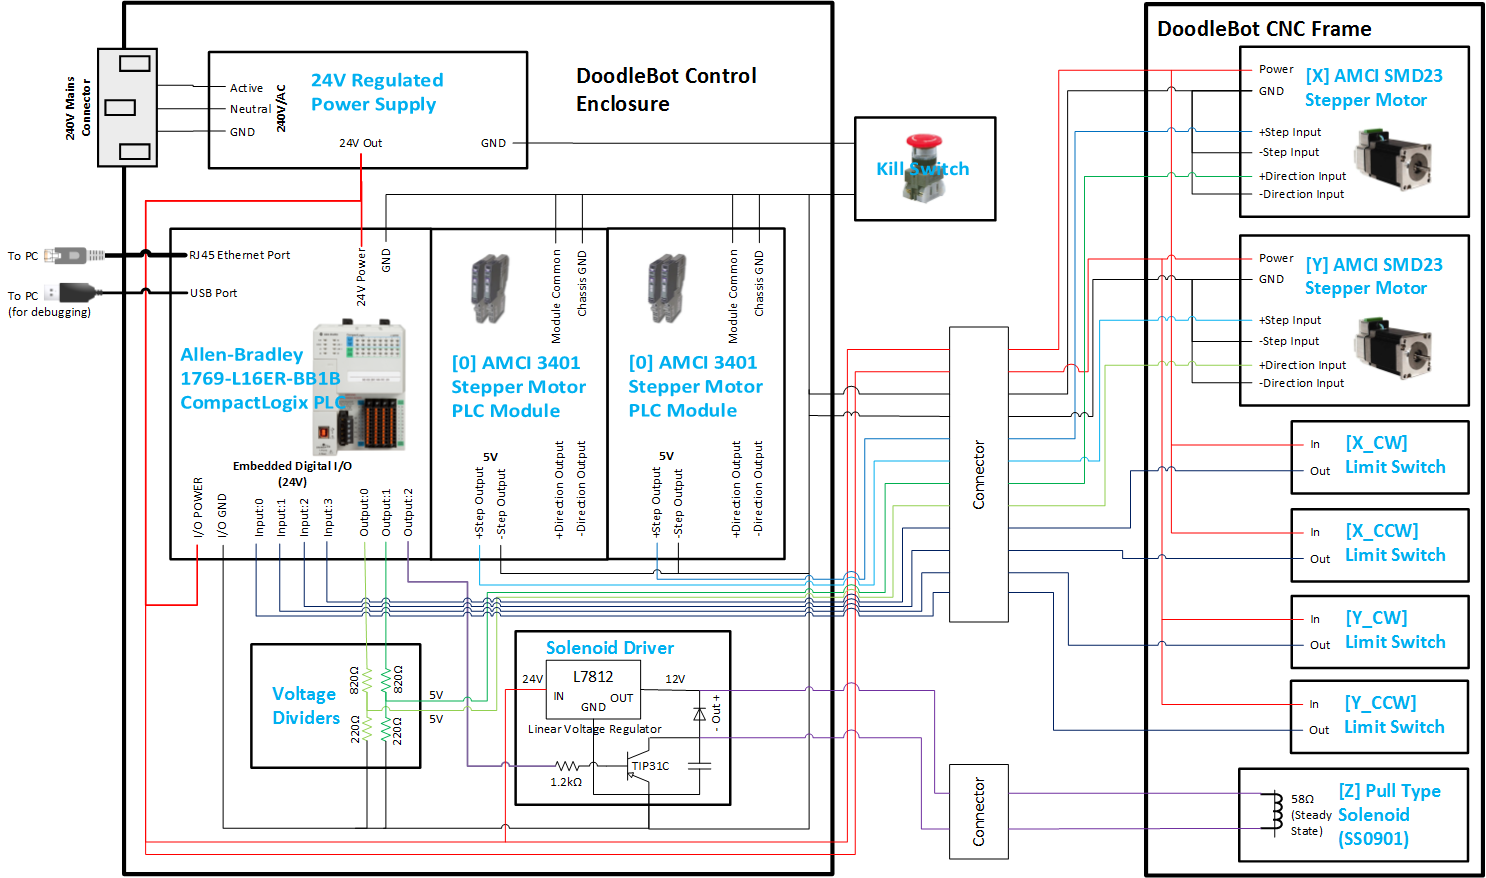
\includegraphics[width=\hsize]{figures/cncMachine/wiring}
		\captionof{figure}{Wiring Diagram}
		\label{fig:WiringDiagram}
		\vspace*{\fill}
\end{landscape}